\title{Parallel Programming Assignment 2: Game of Life Scaling Study on the Blue Gene/Q}
\author{
        %\large
        \textsc{Caitlin Ross}
  %          \qquad
     %   \textsc{}
        \mbox{}\\ %
        Department of Computer Science\\
        CSCI 6360\\
         \\
        \mbox{}\\ %
        \normalsize
            \texttt{rossc3}
     %   \textbar{}
        %    \texttt{yogi}
        \normalsize
            \texttt{@rpi.edu}
}
\date{\today}
\documentclass[11pt]{article}
%\documentclass{acmconf}

\usepackage[paper=a4paper,dvips,top=1.5cm,left=1.5cm,right=1.5cm,
    foot=1cm,bottom=1.5cm]{geometry}

\usepackage{times}
%\usepackage{graphicx}
\usepackage[fleqn]{amsmath}
\usepackage{amsfonts}
\usepackage{amssymb}
\usepackage{amsthm}
\usepackage{amsopn}
\usepackage{xspace}
\usepackage{array}
\usepackage{epsfig}

\numberwithin{figure}{section}

\newcommand\CC{\Lang{\mbox{C++}}\xspace}
\newcommand\Lang[1]{\textsc{#1}}
\newcommand{\kw}[1]{\texttt{\textbf{#1}}}
\newcommand{\cd}[1]{\texttt{#1}}

\newcommand\Naturals{\ensuremath{\mathbb{N}}\xspace}
\newcommand\Integers{\ensuremath{\mathbb{Z}}\xspace}
\newcommand\Rationals{\ensuremath{\mathbb{Q}}\xspace}
\newcommand\Reals{\ensuremath{\mathbb{R}}\xspace}
\newcommand\Complex{\ensuremath{\mathbb{C}}\xspace}

\newcommand\norm[1]{\ensuremath{\lVert#1\rVert}}
\newcommand\abs[1]{\ensuremath{\lvert#1\rvert}}
\newcommand\ceil[1]{\ensuremath{\lceil#1\rceil}}
\newcommand\floor[1]{\ensuremath{\lfloor#1\rfloor}}
\newcommand\set[1]{\ensuremath{\{#1\}}}
\newcommand\angular[1]{\ensuremath{\langle#1\rangle}}

\newcommand\Norm[1]{\ensuremath{\left\lVert#1\right\rVert}}
\newcommand\Abs[1]{\ensuremath{\left\lvert#1\right\rvert}}
\newcommand\Ceil[1]{\ensuremath{\left\lceil#1\right\rceil}}
\newcommand\Floor[1]{\ensuremath{\left\lfloor#1\right\rfloor}}
\newcommand\Set[1]{\ensuremath{\left\{#1\right\}}}
\newcommand\Angular[1]{\ensuremath{\left\langle#1\right\rangle}}

\newcommand{\LOOM}{\ensuremath{\cal{LOOM}}\xspace}
\newcommand{\PolyTOIL}{\textbf{PolyTOIL}\xspace}

\newtheorem{theorem}{Theorem}[section]
\newtheorem{definition}[theorem]{Definition}
\newtheorem{lemma}[theorem]{Lemma}
\newtheorem{corollary}[theorem]{Corollary}
\newtheorem{fact}[theorem]{Fact}
\newtheorem{example}[theorem]{Example}

\newcommand\Cls[1]{\textsf{#1}}
\newcommand\Fig[1]{Figure~\ref{Figure:#1}}

\usepackage{labels} %
%\usepackage{equation}
%\usepackage{prog2tex}

\newenvironment{excerpt}{\begin{quote}\begin{minipage}\textwidth}{\end{minipage}\end{quote}}

\setcounter{topnumber}{0}
\setcounter{bottomnumber}{0}
\setcounter{totalnumber}{20}
\renewcommand{\textfraction}{0.01}

\begin{document}
\newgeometry{margin=1in}

\maketitle

\section{Scaling Study}
This assignment is to run the parallel Game of Life code on the Blue Gene/Q at the CCI and perform a strong scaling performance study.  All experiments for this assignment are performed on a 8192x8192 cell universe with 100 ticks.   In the first series of experiments, the runs are performed with 64 MPI ranks per node.  The number of ranks range from 64 to 8192 by powers of 2, which is 1 to 128 BG/Q nodes.  This set is performed for thresholds of 0\%, 25\%, 50\%, and 75\%.  The execution times are plotted in Figure \ref{fig:scaling}.  From 64 to 1024 MPI ranks, the execution time slightly decreases as the threshold increases.  This trend flips when there are 2048 or more MPI ranks.  The  Tables 1-4 show the speedups and parallel efficiencies for each of these runs based on the 64-rank run.  The speedups are also plotted in Figure \ref{fig:speedup}.  The max speedup is seen when the threshold is 0\% running on 8192 MPI ranks with approximately 89x speedup over the 64-rank case.  The best parallel efficiency is 111\%, which is seen for the case where the threshold is 75\% running on 128 ranks.  As can be seen by looking at the parallel efficiency listed for each case, the speed up is super-linear for each rank count through 1024.  The cause of the super-linear speedup is likely because the problem size is small enough that most of the needed data fits in the cache.  The cause of sub-linear is likely due to the increase of communication relative to the amount of rows each rank is responsible for.  With 2048 MPI ranks, each rank works on 4 rows, whereas at 8192, each rank works on 1 row, meaning it must always communicate with other ranks in order to process its row.  

\begin{center}
\begin{table}[h]
\begin{tabular}{| l | r | r | }
\hline
MPI Ranks & Speedup & Parallel Efficiency \\ \hline
128 & 2.110828 & 1.055414 \\ \hline
256 & 4.198896 & 1.049724 \\ \hline
512 & 8.253606 & 1.031701 \\ \hline
1024 & 16.333831 & 1.020864 \\ \hline
2048 & 28.951401 & 0.904731 \\ \hline
4096 & 51.422706 & 0.803480 \\ \hline
8192 & 88.643905 & 0.692531 \\ \hline
\end{tabular}
\caption{Speedup and Parallel Efficiency of parallel runs relative to 64 MPI rank run for 0\% threshold}
\label{speedup1}

\begin{tabular}{| l | r | r | }
\hline
MPI Ranks & Speedup & Parallel Efficiency \\ \hline
128 & 2.124607 & 1.062304 \\ \hline
256 & 4.230943 & 1.057736 \\ \hline
512 & 8.353213 & 1.044152 \\ \hline
1024 & 16.282762 & 1.017673 \\ \hline
2048 & 28.353092 & 0.886034 \\ \hline
4096 & 48.927447 & 0.764491 \\ \hline
8192 & 83.894824 & 0.655428 \\ \hline
\end{tabular}
\caption{Speedup and Parallel Efficiency of parallel runs relative to 64 MPI rank run for 25\% threshold}

\begin{tabular}{| l | r | r | }
\hline
MPI Ranks & Speedup & Parallel Efficiency \\ \hline
128 & 2.172604 & 1.086302 \\ \hline
256 & 4.333228 & 1.083307 \\ \hline
512 & 8.514183 & 1.064273 \\ \hline
1024 & 16.721624 & 1.045102 \\ \hline
2048 & 27.094837 & 0.846714 \\ \hline
4096 & 47.000365 & 0.734381 \\ \hline
8192 & 80.495623 & 0.628872 \\ \hline
\end{tabular}
\caption{Speedup and Parallel Efficiency of parallel runs relative to 64 MPI rank run for 50\% threshold}

\begin{tabular}{| l | r | r | }
\hline
MPI Ranks & Speedup & Parallel Efficiency \\ \hline
128 & 2.226770 & 1.113385 \\ \hline
256 & 4.417488 & 1.104372 \\ \hline
512 & 8.748572 & 1.093571 \\ \hline
1024 & 16.915214 & 1.057201 \\ \hline
2048 & 26.031290 & 0.813478 \\ \hline
4096 & 44.891403 & 0.701428 \\ \hline
8192 & 76.800630 & 0.600005 \\ \hline
\end{tabular}
\caption{Speedup and Parallel Efficiency of parallel runs relative to 64 MPI rank run for 75\% threshold}

%\begin{tabular}{| l | r | r | }
%\hline
%MPI Ranks & Speedup & Parallel Efficiency \\ \hline
%64 & 2.062819 & 1.031410 \\ \hline
%128 & 4.120698 & 1.030174 \\ \hline
%256 & 8.206570 & 1.025821 \\ \hline
%512 & 16.329667 & 1.020604 \\ \hline
%1024 & 31.979921 & 0.999373 \\ \hline
%2048 & 55.693584 & 0.870212 \\ \hline
%4096 & 86.670136 & 0.677110 \\ \hline
%\end{tabular}
%\caption{Speedup and Parallel Efficiency of parallel runs relative to 32 MPI rank run for 50\% threshold}
\end{table}
\end{center} 

\begin{figure}[t]
\centering
   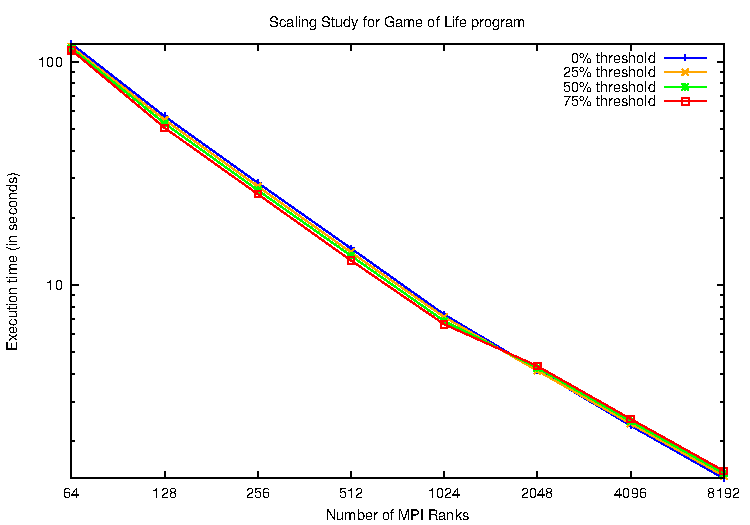
\includegraphics{data/scaling-64.pdf}
\caption{Scaling study performed for 8192x8192 cell universe and 100 ticks at four different threshold levels plotted on log scales for both axes.}
\label{fig:scaling}
\end{figure}
\begin{figure}[t]
\centering
   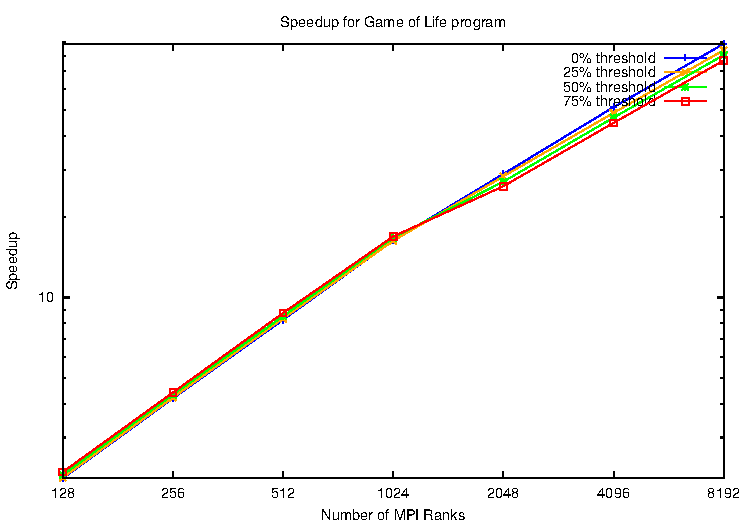
\includegraphics{data/speedup.pdf}
\caption{Speedup observed in scaling study performed for 8192x8192 cell universe and 100 ticks at four different threshold levels plotted on log scales for both axes.}
\label{fig:speedup}
\end{figure}

   
For the next set of experiments, I ran a 8192x8192 cell universe with 100 ticks and a threshold of 50\%.  This is performed with only 32 ranks per node instead of 64, thus the total ranks used range from 32 to 4096.  This is compared to the 64 rank per node case ran with a 50\% threshold described earlier.  The execution times of these runs as a function of the number of nodes are shown in Figure \ref{fig:scaling50}.  In every case the 64 task/node case is faster than the 32 task/node case, since it's running with more total MPI ranks, however at 32 nodes and beyond, the difference between the two is smaller than for a lower number of nodes.  This point corresponds with the turning point of 2048 in the previous set of experiments where performance becomes sub-linear.  
\begin{figure}[t]
\centering
   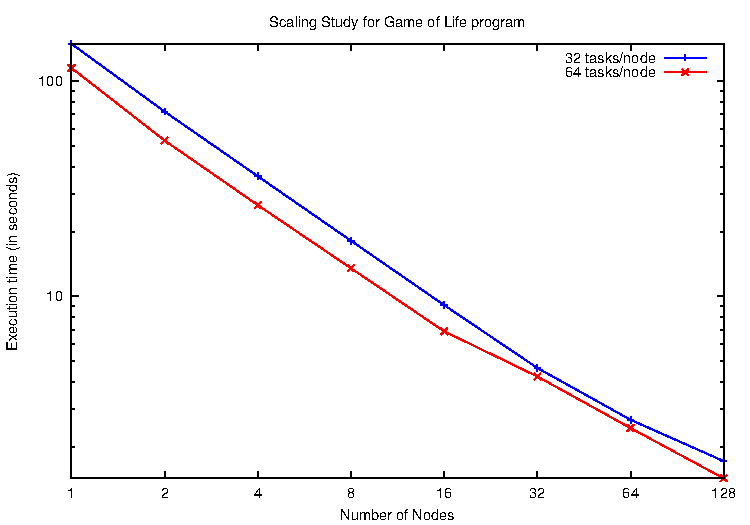
\includegraphics{data/scaling-t50-2.pdf}
\caption{Comparison of using 32 vs 64 tasks per BG/Q node for 8192x8192 cell universe, 100 ticks, and 50\% threshold plotted on log scales for both axes. This is plotted as a function of the number of BG/Q nodes.}
\label{fig:scaling50}
\end{figure}

%\begin{figure}[t]
%\centering
%   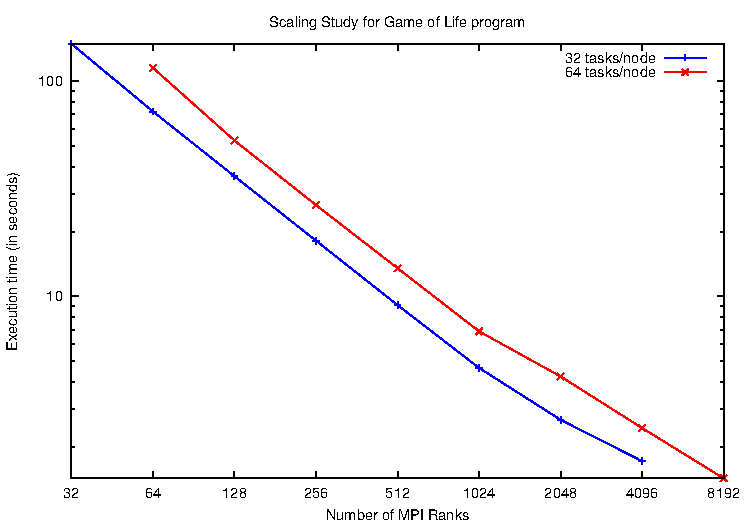
\includegraphics{data/scaling-t50.pdf}
%\caption{Comparison of using 32 vs 64 tasks per BG/Q node for 8192x8192 cell universe, 100 ticks, and 50\% threshold plotted on log scales for both axes. This is plotted as a function of the number of MPI ranks.}
%\label{fig:scaling50}
%\end{figure}







%\bibliography{main}

%\bibliographystyle{abbrv}
\end{document}
